\section{Результаты исследования}

\subsection{VIF-фильтр и отбор состояний}

После VIF-фильтрации остались следующие причины: среднегодовой доход, объем
потребленного алкоголя, количество членов семьи, количество лет образования,
доля дохода на продовольствие, коэффициент Джини сообщества, охват беспроводной
связи и число смертей от вирусных и респираторных заболеваний. Максимальный VIF
после фильтрации не превышал $5{,}01$.

\begin{table}[H]
\centering
\begin{tblr}{colspec={|X[3,l]|X[c]|X[c]|}, row{1}={gray!30,font=\bfseries}, row{even}={gray!10}, hlines, vlines}
Состояние & Spearman & $p$-value \\
Оценка социальной поддержки & 0,7661 & 0,0000 \\
Чувство технологического прогресса & 0,7213 & 0,0000 \\
Индекс кредитного оптимизма & 0,7035 & 0,0000 \\
Индекс продовольственной безопасности & 0,6014 & 0,0000 \\
Индекс семьи & 0,5530 & 0,0000 \\
Чувство неравенства доходов в обществе & -0,3788 & 0,0000 \\
\end{tblr}
\caption{Состояния с наибольшей связью с рангом счастья}
\label{tab:spearman_states}
\end{table}

\begin{figure}[H]
    \centering
    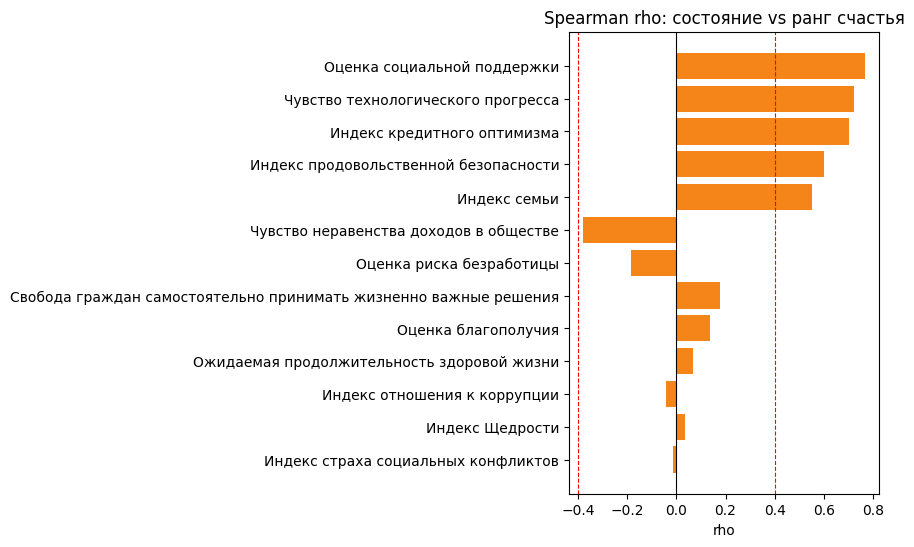
\includegraphics[width=0.76\textwidth]{images/spearman_states.png}
    \caption{Ранговые корреляции состояний с рангом счастья}
    \label{fig:spearman_states}
\end{figure}

Первые четыре состояния не только сильно связаны со счастьем, но и достаточно
хорошо восстанавливаются по причинам. \textit{Индекс семьи} имеет заметную
корреляцию с целевой переменной, но не проходит порог качества восстановления
после выбранной схемы проверки, поэтому в финальный классификатор не включался.

\subsection{Качество восстановления состояний}

\begin{table}[H]
\centering
\begin{tblr}{colspec={|X[3,l]|X[c]|X[c]|X[c]|}, row{1}={gray!30,font=\bfseries}, row{even}={gray!10}, hlines, vlines}
Состояние & Линейный $R^2_{train}$ & После банка функций & $\Delta R^2$ \\
Оценка социальной поддержки & 0,9193 & 0,9301 & 0,0108 \\
Индекс продовольственной безопасности & 0,9172 & 0,9276 & 0,0104 \\
Чувство технологического прогресса & 0,8924 & 0,9183 & 0,0259 \\
Индекс кредитного оптимизма & 0,7929 & 0,9161 & 0,1232 \\
\end{tblr}
\caption{Качество восстановления финально выбранных состояний}
\label{tab:state_r2}
\end{table}

\begin{figure}[H]
    \centering
    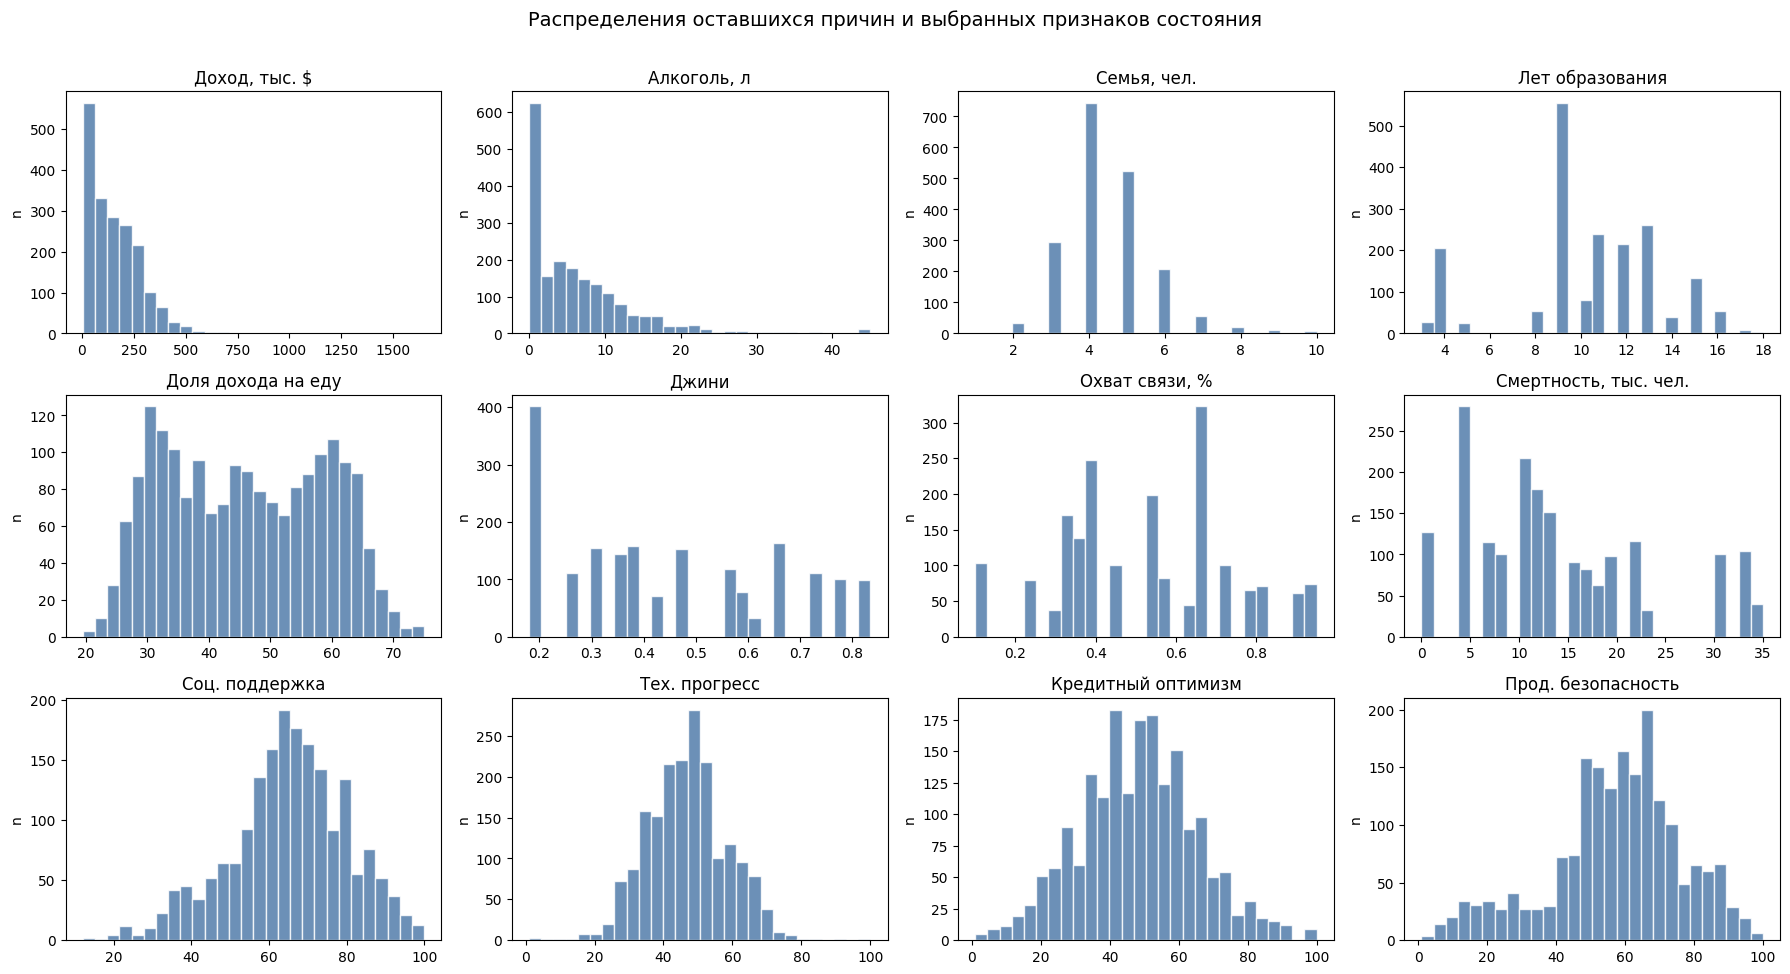
\includegraphics[width=0.96\textwidth]{images/feature_distributions.png}
    \caption{Распределения причин после VIF-фильтра и выбранных состояний}
    \label{fig:feature_distributions}
\end{figure}

Среднее OOF $R^2$ восстановления четырех состояний в проверочном запуске
составило $0{,}9148$. Самым сложным состоянием был индекс кредитного оптимизма:
для него линейная модель без банка функций давала заметно более низкое качество,
а линеаризованные признаки позволили пройти порог отбора.

\subsection{Нелинейности и сообщества}

Наиболее заметная диагностированная нелинейность возникла для связи количества
лет образования с индексом кредитного оптимизма. LOWESS-кривая показывает
монотонный рост с насыщением на больших значениях образования, поэтому
логарифмические и корневые преобразования выглядят содержательно оправданными.

\begin{figure}[H]
    \centering
    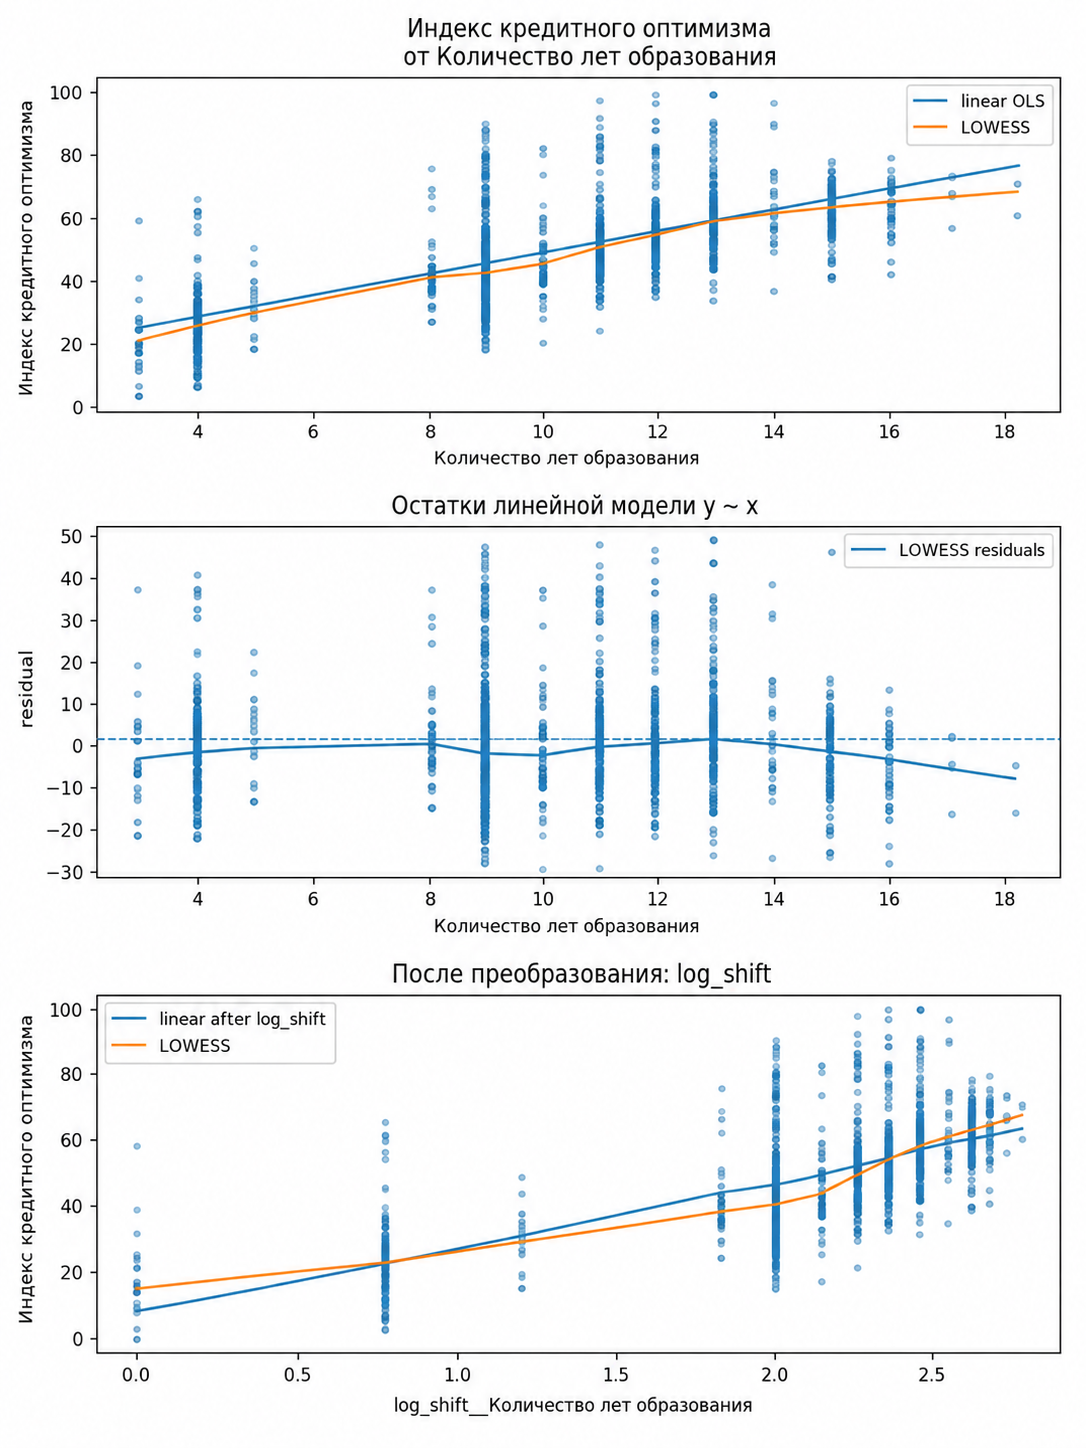
\includegraphics[width=0.98\textwidth]{images/cell8_out0.png}
    \caption{Диагностика нелинейности: индекс кредитного оптимизма и годы образования}
    \label{fig:lowess_education}
\end{figure}

\begin{table}[H]
\centering
\small
\begin{tblr}{
    colspec={|X[2.1,l]|X[2.0,l]|X[0.85,c]|X[0.75,c]|X[0.75,c]|X[0.85,c]|},
    row{1}={gray!30,font=\bfseries},
    row{even}={gray!10},
    hlines,
    vlines
}
Состояние & Причина & Функция & Баз. $R^2$ & Нов. $R^2$ & $\Delta R^2$ \\
Индекс кредитного оптимизма & Количество лет образования & log\_shift & 0,9173 & 0,9208 & 0,0035 \\
Индекс кредитного оптимизма & Количество лет образования & sqrt\_shift & 0,9173 & 0,9207 & 0,0034 \\
Индекс кредитного оптимизма & Количество лет образования & inv\_shift & 0,9173 & 0,9207 & 0,0034 \\
Индекс кредитного оптимизма & Количество лет образования & z4 & 0,9173 & 0,9204 & 0,0031 \\
Индекс кредитного оптимизма & Количество лет образования & log1p & 0,9173 & 0,9204 & 0,0031 \\
Индекс кредитного оптимизма & Количество лет образования & cbrt & 0,9173 & 0,9204 & 0,0031 \\
Индекс семьи & Среднегодовой доход, тыс. \$ & z2 & 0,4727 & 0,4742 & 0,0015 \\
\end{tblr}
\caption{Лучшие одиночные нелинейные преобразования}
\label{tab:linearization}
\end{table}

В таблице~\ref{tab:linearization} показаны лучшие одиночные преобразования,
проверенные отдельно. Их индивидуальный прирост невелик, однако в совокупности
банк функций оказался полезен для восстановления индекса кредитного оптимизма,
что видно по таблице~\ref{tab:state_r2}.

\begin{figure}[H]
    \centering
    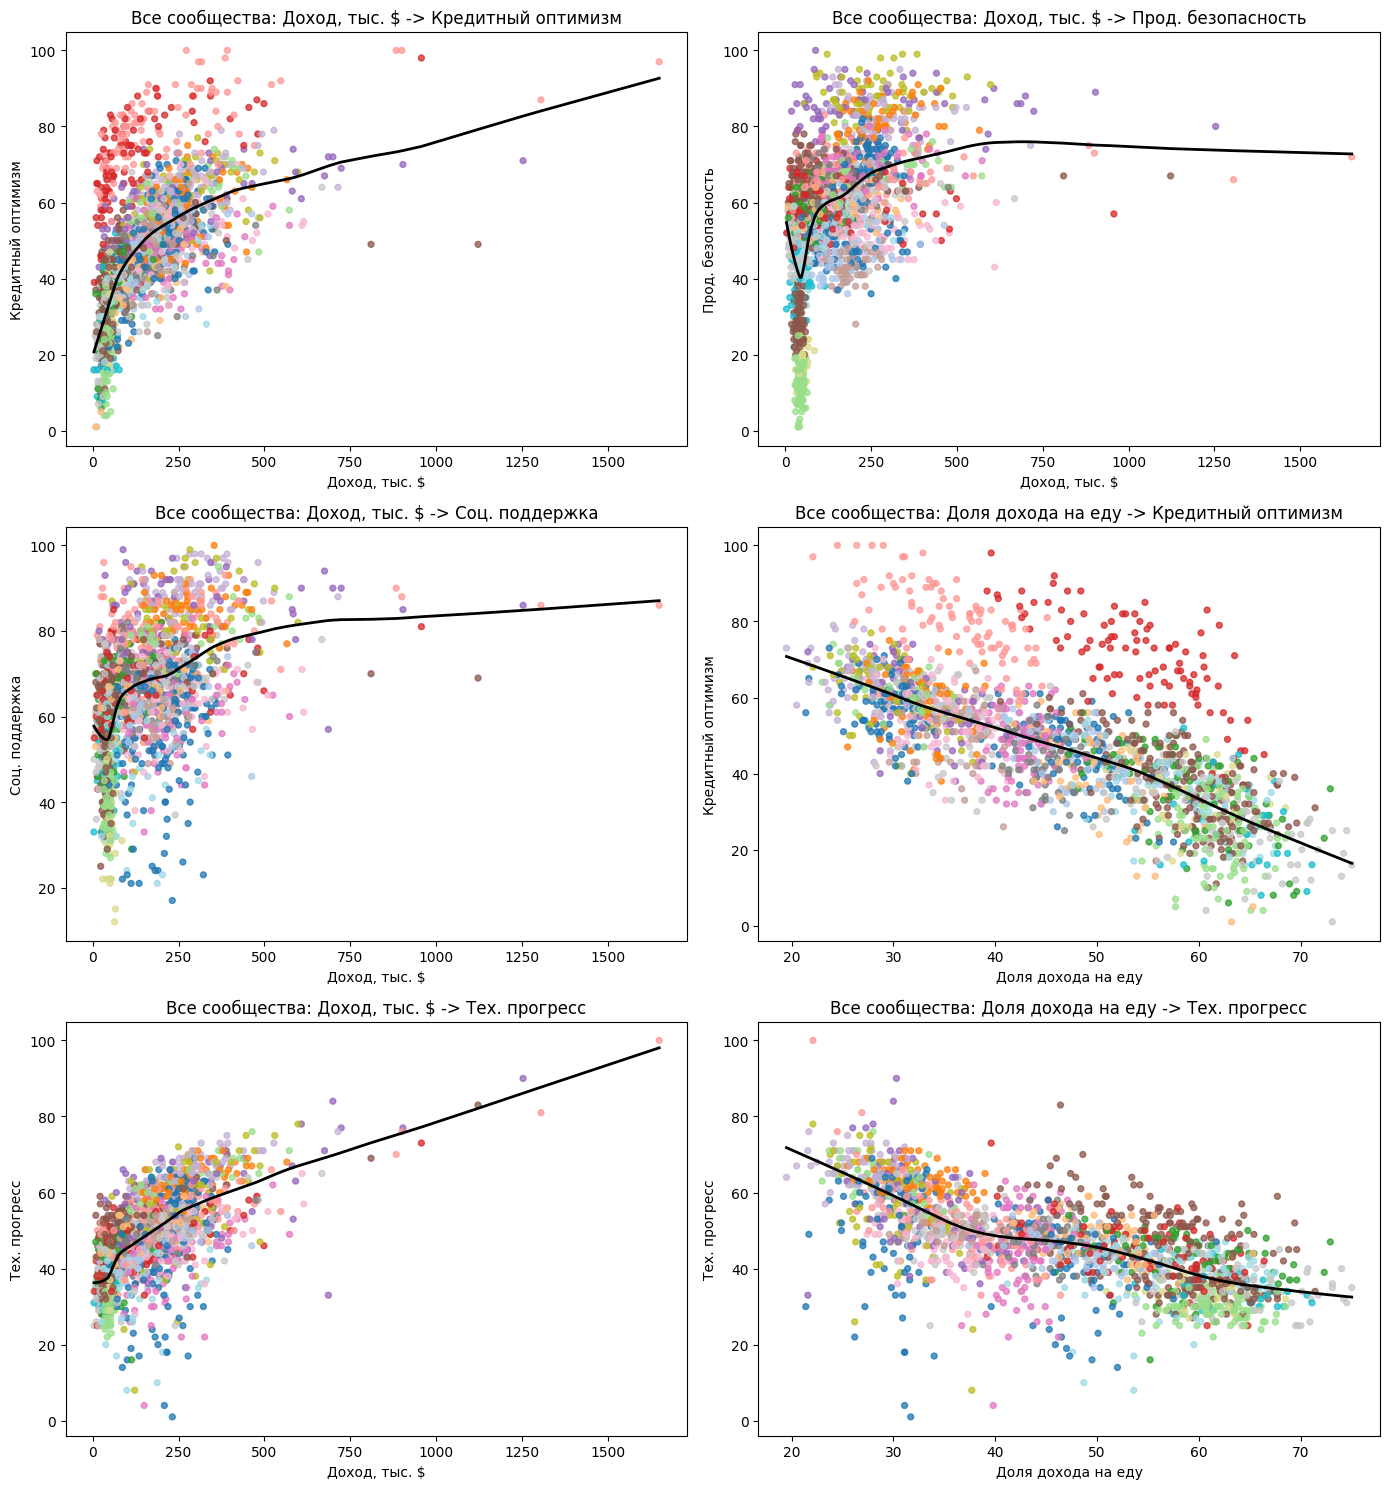
\includegraphics[width=0.96\textwidth]{images/all_communities_scatter.png}
    \caption{Нелинейные зависимости причин и состояний с раскраской по сообществам}
    \label{fig:all_communities_scatter}
\end{figure}

Отдельно были построены графики зависимостей с выделением одного сообщества
красным цветом. Они показывают, что общественные причины задают положение
сообщества как группы, а индивидуальные причины объясняют разброс респондентов
внутри этой группы. Поэтому \code{community\_id} является важным диагностическим
признаком структуры данных, даже если его one-hot-представление не вошло в
финальный классификатор.

\begin{figure}[H]
    \centering
    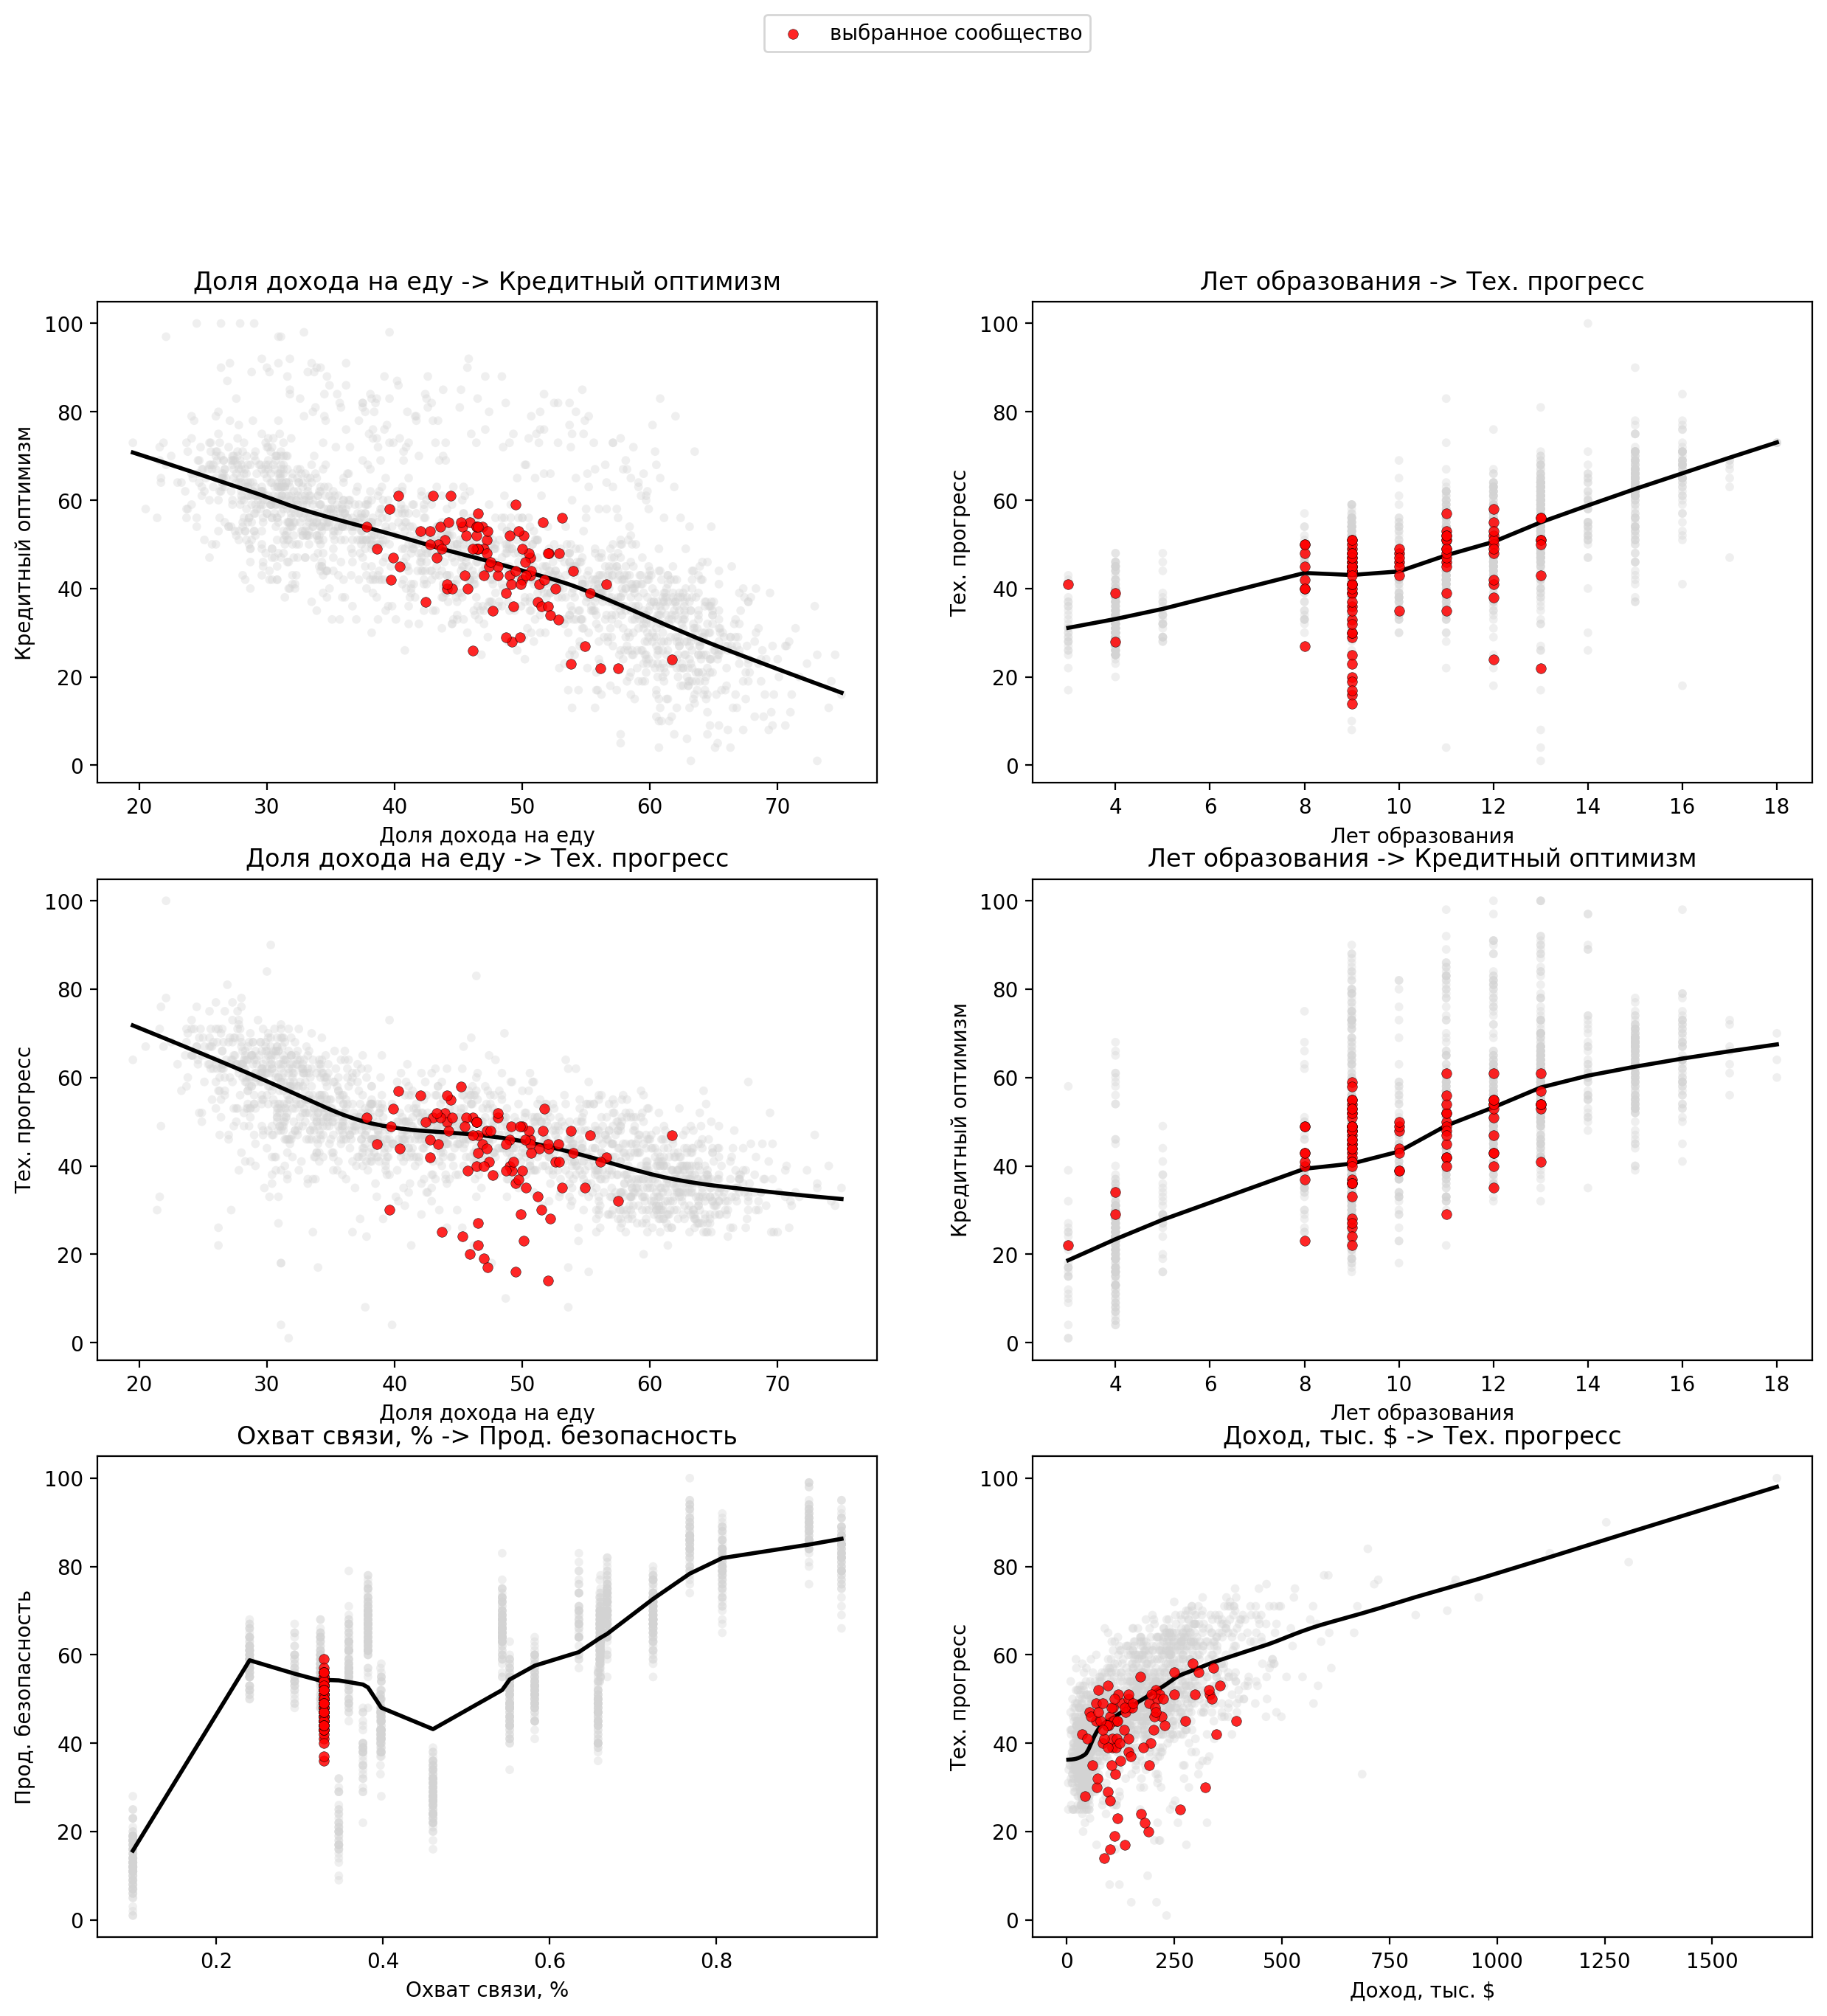
\includegraphics[width=0.92\textwidth]{images/community_001.png}
    \caption{Пример зависимостей с выделением одного сообщества}
    \label{fig:community_scatter}
\end{figure}

\begin{figure}[H]
    \centering
    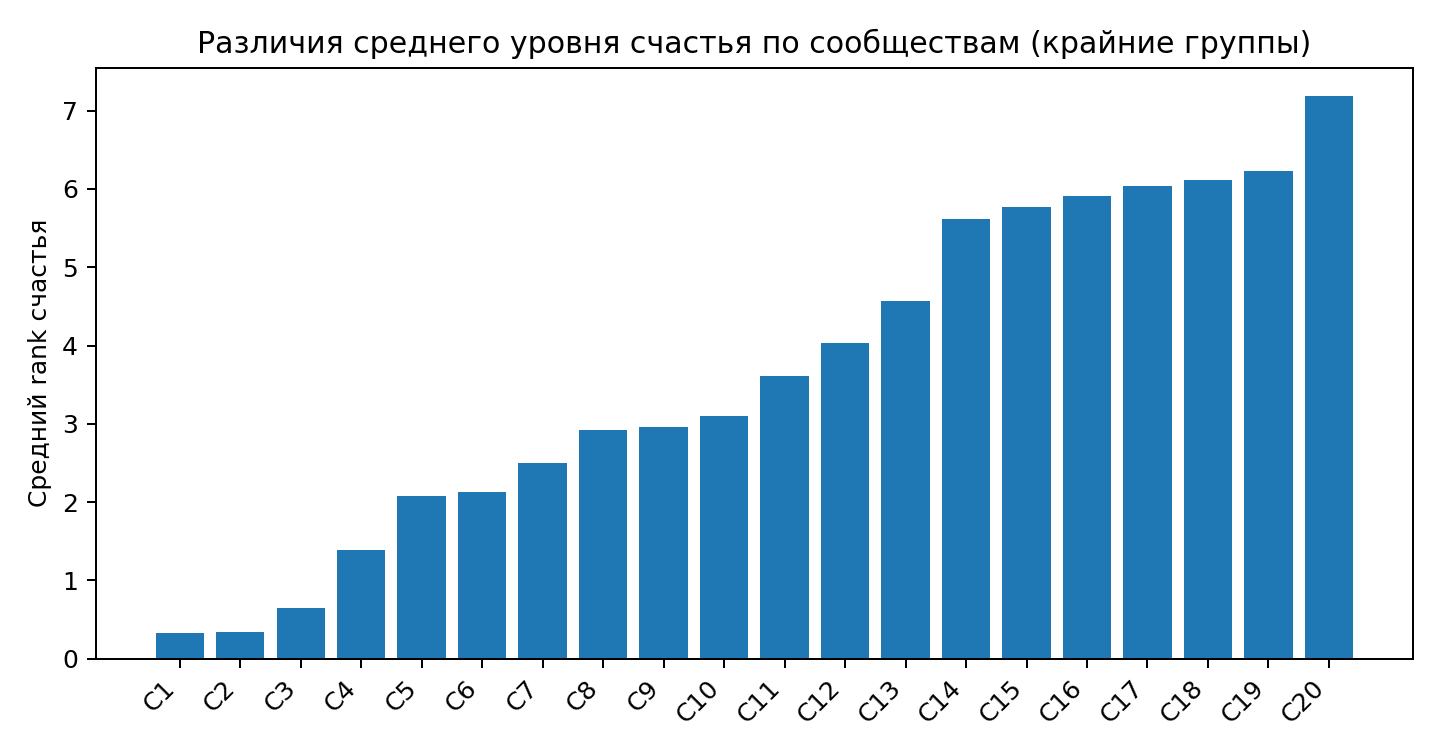
\includegraphics[width=0.90\textwidth]{images/community_mean_rank.png}
    \caption{Различия среднего ранга счастья между сообществами}
    \label{fig:community_rank}
\end{figure}

\subsection{Качество классификации}

Финальная проверка выполнялась на rowwise-разбиении с \code{SEED = 7}. Лучший
воспроизводимый результат дала конфигурация:
\begin{center}
\code{predicted states + vif\_causes + sphere, без community one-hot}.
\end{center}

Итоговое значение micro precision равно $0{,}6063$, что превышает требуемый
порог $0{,}6$. Так как задача является многоклассовой однометочной
классификацией, accuracy имеет то же значение $0{,}6063$.

\begin{table}[H]
\centering
\begin{tblr}{colspec={|X[l]|X[c]|X[c]|X[c]|X[c]|}, row{1}={gray!30,font=\bfseries}, row{even}={gray!10}, hlines, vlines}
Класс & Precision & Recall & F1 & Support \\
Hopeless & 0,74 & 0,79 & 0,76 & 53 \\
Depressed & 0,75 & 0,69 & 0,72 & 55 \\
Suffering & 0,44 & 0,39 & 0,41 & 70 \\
Strugglng & 0,34 & 0,34 & 0,34 & 47 \\
Coping & 0,47 & 0,42 & 0,44 & 65 \\
Just ok & 0,55 & 0,60 & 0,57 & 52 \\
Doing well & 0,73 & 0,88 & 0,80 & 66 \\
Blooming & 0,67 & 0,74 & 0,71 & 39 \\
Thriving & 0,90 & 0,69 & 0,78 & 26 \\
Prospering & 0,67 & 1,00 & 0,80 & 2 \\
\end{tblr}
\caption{Отчет классификации для финальной модели}
\label{tab:classification_report}
\end{table}

\begin{figure}[H]
    \centering
    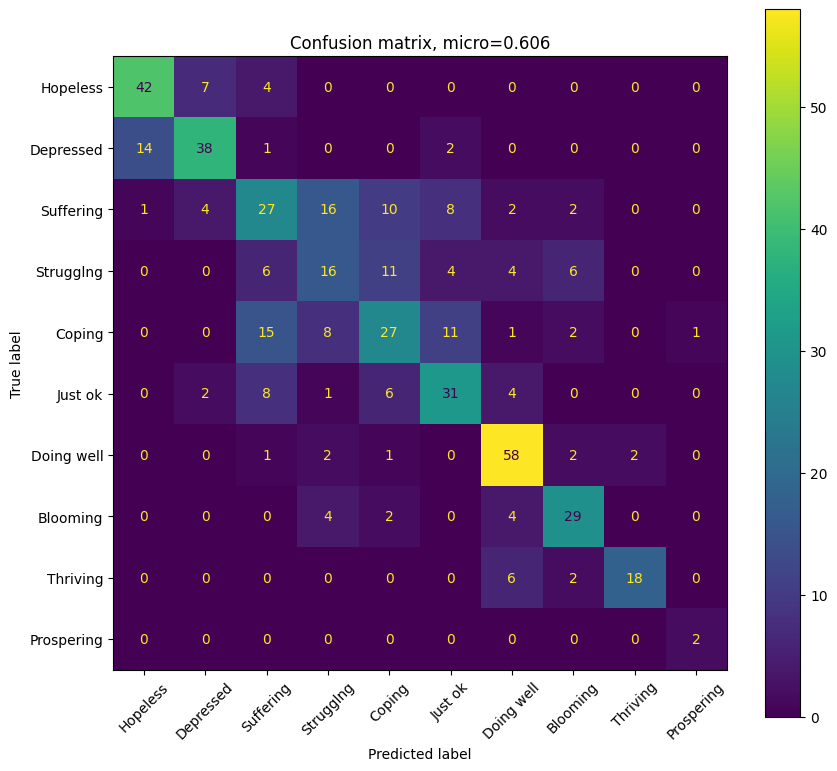
\includegraphics[width=0.86\textwidth]{images/confusion_matrix.png}
    \caption{Матрица ошибок классификатора}
    \label{fig:confusion}
\end{figure}

Матрица ошибок показывает, что основные ошибки возникают между соседними
категориями: \textit{Suffering}, \textit{Strugglng}, \textit{Coping} и
\textit{Just ok}. Для упорядоченной шкалы счастья это ожидаемо: границы между
средними классами менее резкие, чем между крайними состояниями.

\subsection{Прогноз для unknown-наблюдений}

После проверки финальная модель была обучена на всех 1900 known-наблюдениях и
применена к 600 unknown-строкам. Для unknown сначала были восстановлены четыре
состояния, затем по ним, причинам и сфере занятости был предсказан класс
счастья.

\begin{table}[H]
\centering
\begin{tblr}{colspec={|X[l]|X[c]|}, row{1}={gray!30,font=\bfseries}, row{even}={gray!10}, hlines, vlines}
Предсказанный класс & Количество \\
Suffering & 107 \\
Doing well & 98 \\
Hopeless & 71 \\
Just ok & 66 \\
Coping & 63 \\
Strugglng & 62 \\
Depressed & 59 \\
Blooming & 47 \\
Thriving & 24 \\
Prospering & 3 \\
\end{tblr}
\caption{Распределение прогнозов для unknown-наблюдений}
\label{tab:unknown}
\end{table}

\begin{figure}[H]
    \centering
    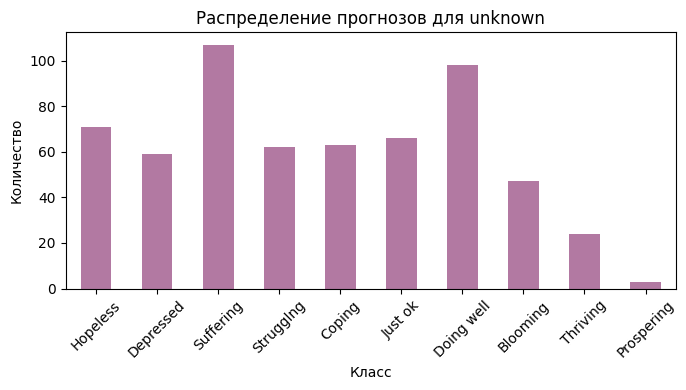
\includegraphics[width=0.85\textwidth]{images/unknown_distribution.png}
    \caption{Распределение предсказанных классов для unknown}
    \label{fig:unknown}
\end{figure}

\newpage
